\subsection{Controlled Scenario Results}
All five scenarios were exercised in both baseline and ANCHOR-managed configurations. Table~\ref{tab:scenario-results} summarizes the completed runs.

\begin{table}[H]
\caption{Controlled Scenario Results}
\label{tab:scenario-results}
\begin{center}
\begin{tabular}{|l|l|c|c|c|}
\hline
Scenario & Mode & Success & Interventions & Notes \\
\hline
Low Battery & Baseline & Yes & 1 & Operator reduced activity manually \\
Low Battery & ANCHOR-managed & Yes & 0 & Local low-power transition, no follow-up needed \\
Geofence Entry & Baseline & Yes & 1 & Operator would need to start mission activity \\
Geofence Entry & ANCHOR-managed & Yes & 0 & Automatic active-mode transition and scan behavior \\
Target Wi-Fi Detection & Baseline & Yes & 1 & Operator must interpret detection \\
Target Wi-Fi Detection & ANCHOR-managed & Yes & 0 & Detection captured without operator action \\
Disconnect & Baseline & No & 1 & Recovery required operator verification \\
Disconnect & ANCHOR-managed & No & 0 & Local continuity preserved, sync resumed after reconnect \\
Command Failure & Baseline & No & 1 & Operator manually marked failure \\
Command Failure & ANCHOR-managed & No & 1 & Managed mode did not improve failure observability \\
\hline
\end{tabular}
\end{center}
\end{table}

Three patterns stand out from these controlled runs. First, ANCHOR-managed mode consistently reduced intervention count in low-battery, geofence-entry, and target-Wi-Fi-detection scenarios. Second, disconnect handling demonstrated graceful degradation and later recovery, but not true autonomous reestablishment of the underlying link. Third, command-failure handling remains a significant limitation of the current prototype, because neither baseline nor ANCHOR-managed mode reliably surfaced a failed command response back into the experiment harness.

\begin{figure}[H]
\begin{center}
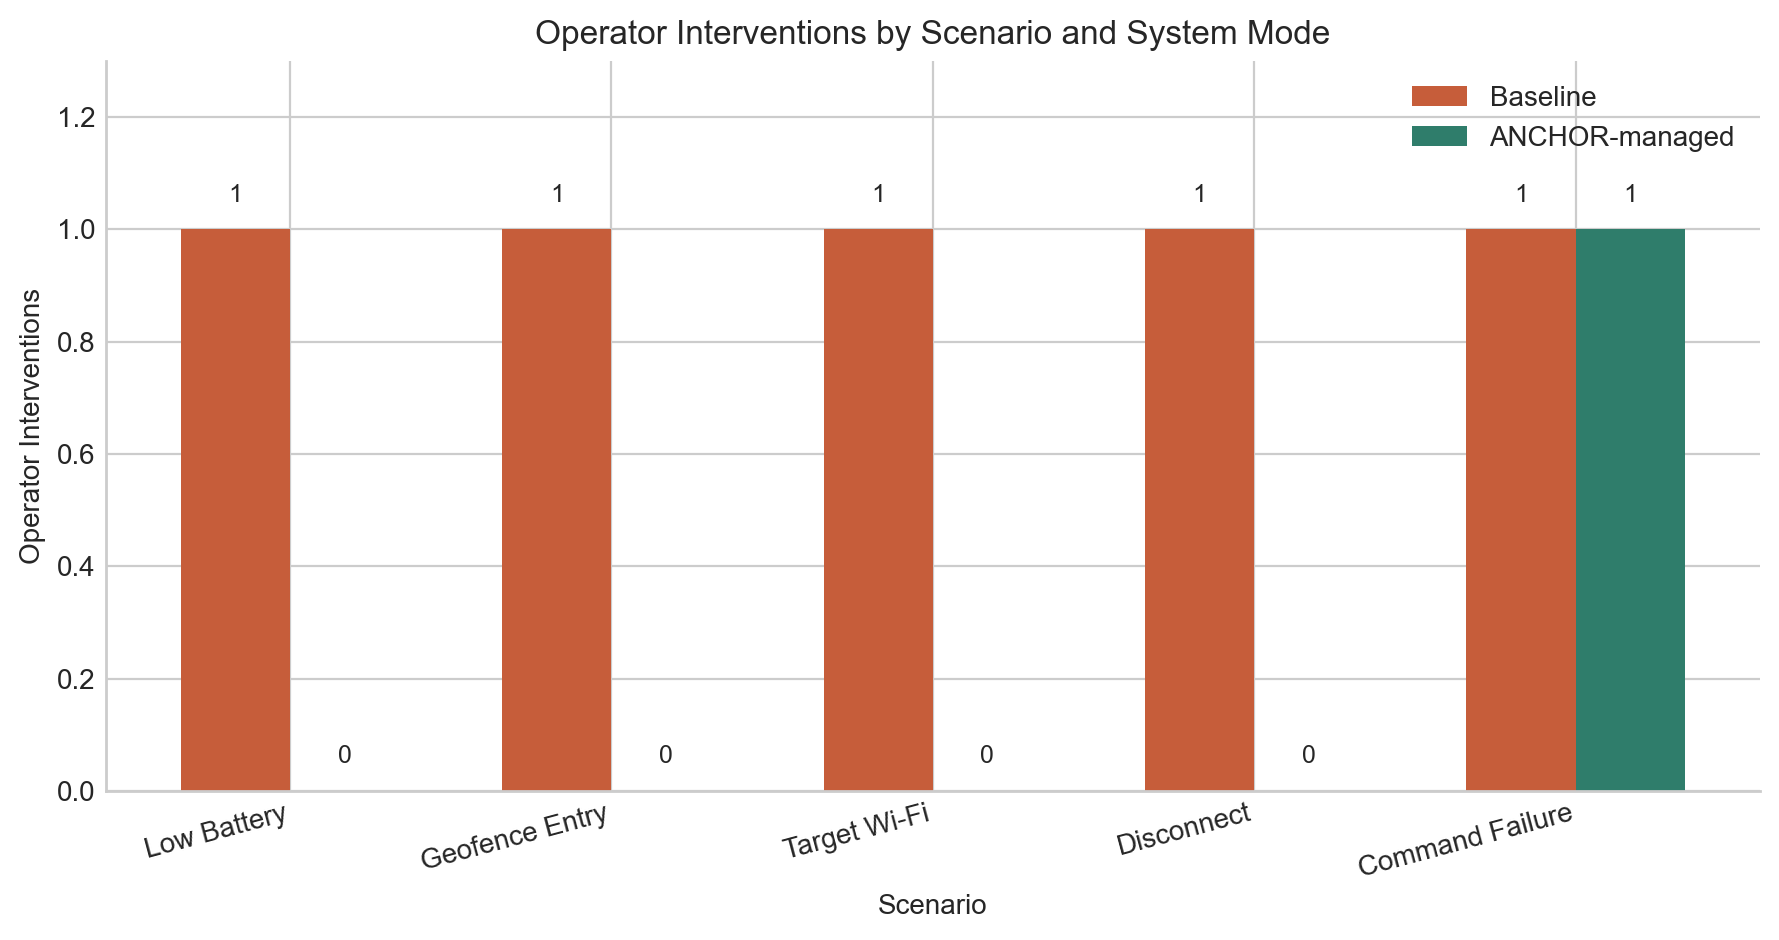
\includegraphics[width=0.48\textwidth]{docs/figures/intervention_bar_chart.png}
\caption{Operator interventions required in each controlled scenario for the baseline and ANCHOR-managed configurations.}
\label{fig:intervention-bar-chart}
\end{center}
\end{figure}
